\documentclass[11pt,letterpaper,boxed]{pset}

\usepackage[margin=0.75in]{geometry}
\usepackage{ulem}

\begin{document}

    \problemlist{PHYS051 HW03}
    \begin{center}
    	  SUP 1A; SUP 2A; *E28.3; SUP 3A; P28.6; P28.10

    \end{center}
    
    \begin{problem} [SUP 1A]
    Suppose an electric field is given by $\Vec{E}=(\frac{k}{r})\hat{r}$ in spherical coordinates, where $k$ is a constant.
    
    \begin{itemize}
        \item [(a)] Find the volume charge density $\rho$.
        \item [(b)] Using Gauss's Law, find the total charge contained in a sphere of radius $R$, centered at the origin (at $r=0$).
        \item [(c)] Repeat part (b), but this time find the total charge by direct integration of $\rho$ over the volume of the sphere.
    \end{itemize}
    \end{problem}
    \newpage
    
    \begin{problem} [SUP 2A]
    A dielectric material of dielectric constant $\kappa_e$ is placed in the interior of the capacitor, shown below. Assume there is a free surface charge $\pm\sigma$ on the plates of the capacitor. What is the polarisation charge induced on each surface of the dielectric $\sigma_{ind}$? Determine your answer using Gauss's Law and the definition of the dielectric constant $\kappa_e=E_0/E_{dielec}$.
    \end{problem}
    \begin{figure*} [ht]
        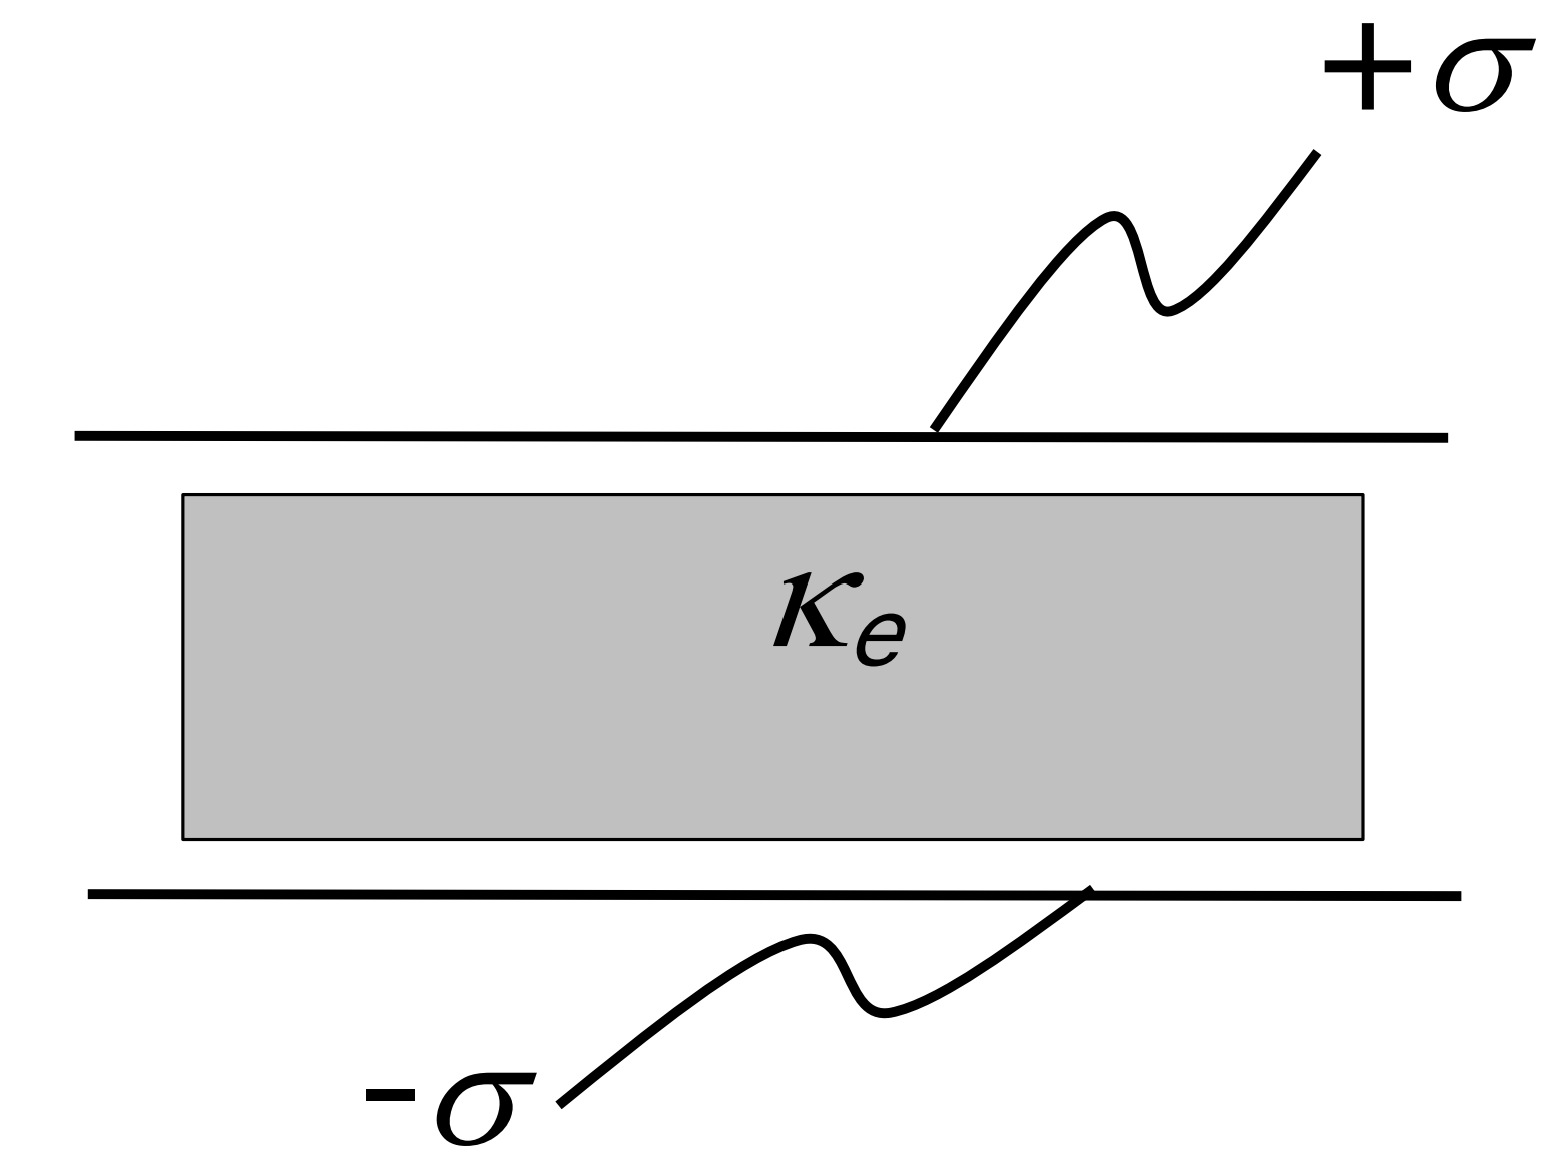
\includegraphics[width=125px]{HW3Images/SUP2A.png}
        \label{fig:P27-4}
    \end{figure*}
    \newpage
    
    \begin{problem} [*E28.3]
    A decade before Einstein published his theory of relativity, J. J. Thomson proposed that the electron might be made up of small parts and that its mass is due to the electrical interaction of the parts. Furthermore, he suggested that the energy equals $mc^2$. Make a rough estimate of the electron mass in the following way: assume that the electron is composed of three identical parts that are brought in from infinity and placed at the vertices of an equilateral triangle having sides equal to the classical radius of the electron, $2.82\cdot10^{-45}$m. 
    \begin{itemize}
        \item [(a)] Find the total electric potential energy of this arrangement. 
        \item [(b)] Divide by $c^2$ and compare your result to the accepted electron mass ($9.11\cdot10^{31}$kg).
        \item [(c)] Did the external agent do work to build the electron, or was work done to the agent by the field?
    \end{itemize}
    The result improves if more parts are assumed; see Problem 2. Today, the electron is thought to be a single, indivisible particle.
    \end{problem}
    \newpage
    
    \begin{problem} [SUP 3A/E28.35]
    The electric potential $V$ in the space between plates of a particular, and now obsolete, vacuum tube is given by $V$=(1530 $V/m^2$)$x^2$, where $x$ is the distance from one of the plates. Calculate the magnitude and direction of the electric field at $x=1.28$cm. Also determine the volume charge density $\rho$ between the plates, and the surface charge density on each of the plates, assuming one plate is at $x = 0$ and the other is at $x = 1.28$ cm. Consider the plates to be metal conductors of finite thickness.
    \end{problem}
    \newpage
    
    \begin{problem} [P28.6]
    A particle of mass $m$, charge $q > 0$, and initial kinetic energy $K$ is projected (from an infinite separation) toward a heavy nucleus of charge $Q$, assumed to have a fixed position in our reference frame.
    
    \begin{itemize}
        \item [(a)] If the aim is "perfect," how close to the center of the nucleus is the particle when it comes instantaneously to rest?
        \item [(b)] With a particular imperfect aim, the particle's closest approach to the nucleus is twice the distance determined in part (a). Determine the speed of the particle at this closest distance of approach. Assume that the particle does not reach the surface of the nucleus.
    \end{itemize}
    \end{problem}
    \newpage
    
    \begin{problem} [P28.10]
    A total amount of positive charge $Q$ is spread onto a nonconducting, flat, circular annulus of inner radius $a$ and outer radius $b$. The charge is distributed so that the charge density (charge per unit area) is given by $\sigma=k/r^3$, where $r$ is the distance from the center of the annulus to any point on it. Show that (with $V=0$ at infinity), the potential at the center of the annulus is given by $$V=\frac{Q}{8\pi\epsilon_0}(\frac{a+b}{ab})$$.
    \end{problem}
    \newpage
\end{document}